documentclass[../PHYS306Notes.tex]{subfiles}

\begin{document}
\subsection{Worksheet - Shortest Distance and Variational Principle}
\begin{p}
We wish to find the shortest path between two points $(x_1,y_1)$ and $(x_2,y_2)$ in the plane. First, write out the distance between these two points in terms of a general function $y(x)$ connecting points $(x_1,y_1)$ and $(x_2,y_2)$, and possibly it’s derivative $y'(x)$, in terms of an independent variable $x$.
\begin{center}
    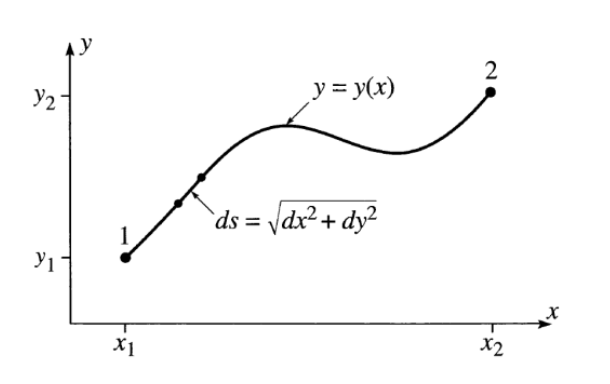
\includegraphics[scale=0.6]{Lecture-1/W1-img1.png}
\end{center}
\end{p}
\begin{s}
We can define an infinitesimal path element of the trajectory from $(x_1, y_1)$ to $(x_2, y_2)$ as:
\[ ds = \sqrt{dx^2 + dy^2}\]
We can use the identity:
\[ dy \equiv \dod{y}{x}dx = y'(x)dx\]
Substituting this into the path element equation above, we obtain:
\[ds = \sqrt{dx^2 + \left(y'(x)dx\right)^2}\]
We may integrate the path element from the initial state to the final state to obtain the length of the path:
\[L(y(x), y'(x)) = \int_{t_1}^{t_2} ds = \int_{x_1}^{x_2} \sqrt{dx^2 + \left(y'(x)dx\right)^2} = \int_{x_1}^{x_2} \sqrt{1 + y'(x)^2}dx\]
Notice here we have the functional $L[y(x), y'(x)]$ (here only depends on $y'(x)$). 


\end{s}

\begin{p}
If light were travelling between points $(x_1,y_1)$ and $(x_2,y_2)$, we would expect it to follow a straight line, but if the index of refraction $n = n(x,y)$ is not constant, the speed of light in the medium is $v = c/n$ and the path is not a straight line but follows the trajectory of minimum time (Fermat, 1662).Find an integral expression for the time taken by a trajectory $y(x)$ through a medium $n(x,y)$.
\end{p}
\begin{s}
The infinitesimal time element $dt$ to travel a distance $ds$ is given by:
\[dt = \frac{ds}{v} = \frac{n(x,y) ds}{c} = \frac{1}{c} n(x,y)\sqrt{1 + y'(x)^2}dx \]
Where in the second inequality we use the identity $v = c/n$. Again we can integrate from an initial time to a final time to obtain the total time the light takes to travel along the path:
\[T = \int_{t_1}^{t_2} dt = \int_{x_1}^{x_2} \frac{1}{c} n(x,y)\sqrt{1 + y'(x)^2}dx = \frac{1}{c}\int_{x_1}^{x_2} n(x,y) \sqrt{1+y'(x)^2}dx\]
Where again we have a functional $T[y(x), y'(x)]$.
\end{s}

\begin{p}
In our variational treatment, if the “wrong” or “varied” curves from the minimum pass through the points 1 and 2, write the condition on the deviations from the correct curve, $\eta(x)$.
\end{p}
\begin{s}
$\eta(x_1) = \eta(x_2) = 0$ as the endpoints of the wrong path must match that of the correct path. 
\end{s}

\begin{p}
If $S(\alpha)=\int_{x_{1}}^{x_{2}} f\left(y+\alpha \eta, y^{\prime}+\alpha \eta^{\prime}, x\right) d x,$ use the chain rule to write $d S(\alpha) / d \alpha$ in terms of an integral of a function that contains derivatives on $y$ and $y^{\prime},$ and $\eta$ and $\eta^{\prime}$.
\end{p}
\begin{s}
As the integral is with respect to x, we may interchange the order of integration and differentiation:
\[\left. \dod{S(\alpha)}{\alpha}\right|_{\alpha = 0} = \left.\dod{}{\alpha}\int_{x_{1}}^{x_{2}} f\left(y+\alpha \eta, y^{\prime}+\alpha \eta^{\prime}, x\right) dx\right|_{\alpha = 0} = \int_{x_1}^{x_2} \left(\left.\dpd{}{\alpha}f\left(y+\alpha \eta, y^{\prime}+\alpha \eta^{\prime}, x\right)\right|_{\alpha = 0}\right) dx \]
Then by the chain rule, we have:
\[\left.\dod{S(\alpha)}{\alpha}\right|_{\alpha = 0} = \int_{x_{1}}^{x_{2}} \left(\eta\dpd{f}{y} + \eta'\dpd{f}{y'}\right)dx = \int_{x_1}^{x_2} \eta\dpd{f}{y} dx + \int_{x_1}^{x_2} \eta'\dpd{f}{y'}dx\]
\end{s}

\begin{p}
Rewrite the $2^{\text {nd }}$ term $\int_{x 1}^{x 2} \eta^{\prime} \frac{\partial f}{\partial y^{\prime}} d x$ by integrating by parts. Note $\int v d u=[u v]-\int u d v$ is equivalent to $\int u^{\prime} v d x=[u v]-\int u v^{\prime} d x$. After simplifying, write the integral expression for $\frac{\partial S}{\partial \alpha}=0 .$ l.e. $\frac{\partial S}{\partial \alpha}= \int_{x 1}^{x 2} \eta(x)[\ldots] d x=0 .$ This condition ensures that $S(\alpha)$ has a minimum at $\alpha=0$ and $y$ is the curve that extremizes S.
\end{p}
\begin{s}
Carrying out integration by parts on the second term, we have:
\[\left. \dod{S(\alpha)}{\alpha}\right|_{\alpha = 0} = \int_{x_1}^{x_2} \eta \dpd{f}{y} dx + \left. \eta\dpd{f}{y'}\right|_{x_1}^{x_2} - \int_{x_1}^{x_2}\eta\left(\dod{}{x}\dpd{f}{y'}\right)dx \]
From problem 3, we know that $\eta(x_1) = \eta(x_2) = 0$ and so the second term evaluates to zero, leaving us with:
\[\left. \dod{S(\alpha)}{\alpha}\right|_{\alpha = 0} = \int_{x_1}^{x_2} \left(\eta\dpd{f}{y} - \eta\dod{}{x}\dpd{f}{y'}\right)dx\]
and we set this to zero:
\[\left. \dod{S(\alpha)}{\alpha}\right|_{\alpha = 0} = \int_{x_1}^{x_2}\eta\left(\dpd{f}{y} - \dod{}{x}\dpd{f}{y'}\right)dx = 0\]
We require that this holds for \textbf{all} possible deviations $\eta(x)$. The only way this could hold is if the term in brackets is zero; this is exactly the Euler-Lagrange equation!
\end{s}

\begin{p}
Write the general form of the Euler-Lagrange Equation. What is the function $f$ for the distance between two points? What does this say about $\pd{f}{y}$ in the E-L equation?
\end{p}
\begin{s}
The general form of the Euler-Lagrange equation is given by:
\[\dpd{f}{y}  - \dod{}{x}\dpd{f}{y'} = 0\]
The function for the distance between two points is $f = \sqrt{1+ y'^2}$ as derived above. Hence, $\dpd{f}{y} = 0$, and therefore by the Euler Lagrange equation:
\[\dpd{f}{y'} = \text{constant}\]
\end{s}

\begin{p}
Solve the above equation for $y'^2$ and hence $y'$ and $y$.
\end{p}
\begin{s}
We have that:
\[\dpd{f}{y'} = \frac{y'}{\sqrt{1+y'^2}} = \text{Constant}\]
Therefore:
\[y'^2 = c^2(1+y'^2)\]
Or alternatively:
\[y'^2 = \frac{c^2}{1-c^2} = c' \implies y'(x) = \sqrt{c'} = m\]
So integrating, we have that:
\[y(x) = mx + b\]
as we knew already!
\end{s}
\end{document}